\section{Potential limits in shared memory programming models} \label{potentialLimits}

In this section two technical aspects that can potentially affect the overall performance of applications conforming to the shared memory programming model are evaluated. The first is related to the performance of the computer's memory sub-system, and the second relates to the cost of the barriers required by parallel programs to ensure correct results.
%\medskip


\subsection*{Stream Benchmark}

For a long time we have witnessed how CPUs are getting faster much more quickly than the computer's memory sub-system. Modern multi-core processors have become voracious consumers of data, and, as a consequence, more and more programs are being limited in performance by the memory bandwidth of the system, rather than by the computational performance of the CPU\cite{McCalpin2007}. It is, therefore, particularly important to be able to determine the memory bandwidth of the system at hand. 

\medskip


The STREAM benchmark\cite{McCalpin2007} is a suite of four simple tests (Copy, Scale, Add and Triad) that measures sustainable memory bandwidth (in MB/s) and the corresponding computation rate for simple vector kernels. In general, it is used to measure the evolution of the memory bandwidth of shared memory systems as more computing components are included in the test. Traditionally, the test has been implemented using OpenMP and the computing components are usually referred as threads.

\medskip

For MPI$_{sm}$ to become a viable alternative to OpenMP in the context of the shared memory programming model, it is fundamental that its sustainable memory bandwidth compares favorably to its OpenMP counterpart.

\medskip

The program that can be downloaded from the stream's website \cite{McCalpin2007} is already annotated with directives (\textbf{\#pragma}) to make it a correct OpenMP program. This program was modified in order to develop an equivalent  MPI$_{sm}$ version. Both programs were run, using various compilers and MPI implementations. Some results, as well as comments on lessons learned, follow.

\medskip

Figure \ref{fig:TriadTestBefore} presents results obtained on one system (\textbf{stout}) for the Triad test of the stream suite; results of the other tests (Copy, Scale and Add) are similar. The left plot (\ref{fig:TriadBefore}) shows the actual achieved bandwidth, while the right plot (\ref{fig:TriadRatioBefore}) shows the MPI$_{sm}$ to OpenMP ratio obtained.
 
\medskip

\begin{figure} [h!]
    \centering
    \captionsetup{justification=centering, singlelinecheck=false}
    \begin{subfigure}{.6\textwidth}
      \hspace*{-1.5cm} 
      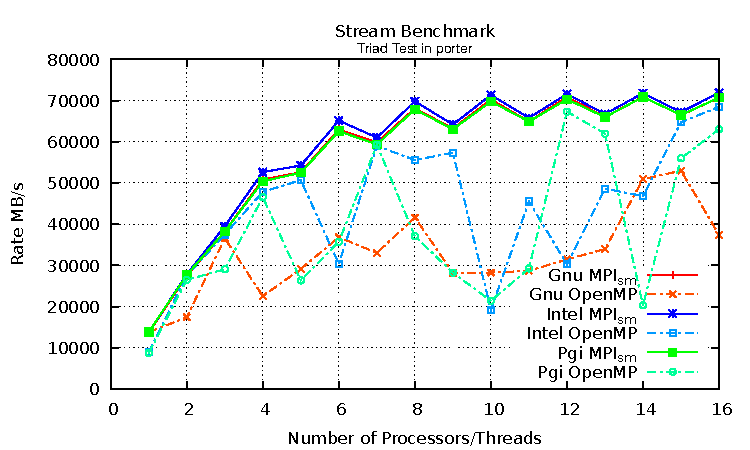
\includegraphics[width=0.95\linewidth]{Plots/streamBenchmark/porter-TriadBefore.pdf}
      \caption[]{Bandwidth per number of processes/threads.}
      \label{fig:TriadBefore}
    \end{subfigure}%
    \begin{subfigure}{.6\textwidth}
      \hspace*{-1.5cm} 
      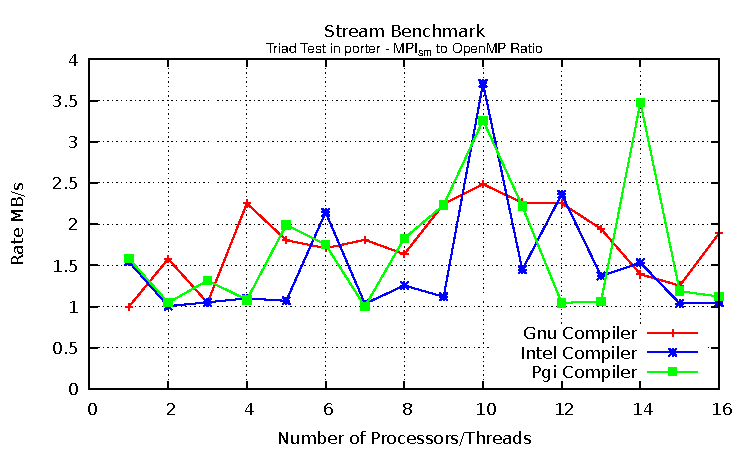
\includegraphics[width=0.95\linewidth]{Plots/streamBenchmark/porter-TriadRatioBefore.pdf}
      \caption{Ratio MPI$_{sm}$ to OpenMP.}
      \label{fig:TriadRatioBefore}
    \end{subfigure}
    \caption{Triad test. No binding policy for OpenMP}
\label{fig:TriadTestBefore}
\end{figure}


In Figure \ref{fig:TriadBefore} the segmented lines correspond to OpenMP while the continuous lines represent MPI$_{sm}$. Notice the extremely irregular behavior shown by all the OpenMP cases. Exploring the causes of such behavior lead to the first lesson in this section: \textbf{thread placement}. As mentioned in Section \ref{introduction}, all the computers used in this study corresponds to systems having more than one socket. In this kind of systems, application having multiple threads could run into affinity problems.

\medskip

The lack of a \emph{by-default} thread affinity control policy of all the compilers used in the study produced the erratic behavior shown in the Figure \ref{fig:TriadBefore} for the OpenMP cases, because the threads are allowed to be moved, by the OS, not only to a different core but also to a different socket. On the other hand, the more stable behavior that can be observed in the MPI$_{sm}$ cases is due to the fact that each of the MPI implementations used in the study indeed has a \emph{by-default} binding policy for the processes running on the node.

\medskip

%The ways to control thread affinity in OpenMP used to be compiler-dependent.

Before the release of the OpenMP version 4.0 specification the mechanisms for controlling thread affinity were compiler-dependent. However, that specification introduced a standardized mean to control thread affinity allowing, for the first time, a uniform way to have fine grain control over the affinity policy to compilers conforming to the standard. Two new concepts were introduced: binding policy and place partition.

\medskip

The binding policy determines if the threads will be bound and how they will be distributed, while the place partition is the set of places to which threads can be bound. Therefore, a simple way of controlling the binding policy is by defining the \textbf{\texttt{OMP\_PROC\_BIND}} environment variable. Similarly, the place partition is set by defining the \textbf{\texttt{OMP\_PLACES}} environment variable.

\medskip

In our case, we found convenient to define:

\begin{itemize} 

\item \textbf{\texttt{OMP\_PROC\_BIND}}=spread 

\item \textbf{\texttt{OMP\_PLACES}}=sockets

\end{itemize}

The above definitions mean that the threads will indeed be bound, and distributed (or spread) among the sockets. More details about the values allowed for these environmental variables can be found in the current OpenMP API specification.

\medskip

Once a thread policy was set for the OpenMP cases, the stream tests were run again and the results are shown in Figure \ref{fig:TriadTest}. As before, the left plot (\ref{fig:Triad}) shows the actual bandwidth achieved while the right plot (\ref{fig:TriadRatio}) shows the MPI$_{sm}$ to OpenMP ratio obtained. 

\medskip
From the results shown in Figure \ref{fig:TriadTest} it can be seen that the sustainable memory bandwidth achievable by MPI$_{sm}$ is effectively at the pair with its OpenMP counterpart.


\begin{figure} [h!]
    \centering
    \captionsetup{justification=centering, singlelinecheck=false}
    \begin{subfigure}{.6\textwidth}
      \centering
      \hspace*{-1.5cm} 
      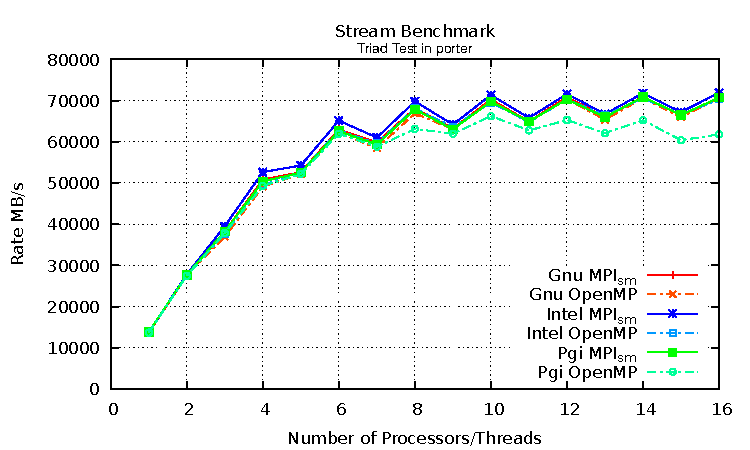
\includegraphics[width=0.95\linewidth]{Plots/streamBenchmark/porter-Triad.pdf}
      \caption[]{Bandwidth per number of processes/threads.}
      \label{fig:Triad}
    \end{subfigure}%
    \begin{subfigure}{.6\textwidth}
      \centering
      \hspace*{-1.5cm} 
      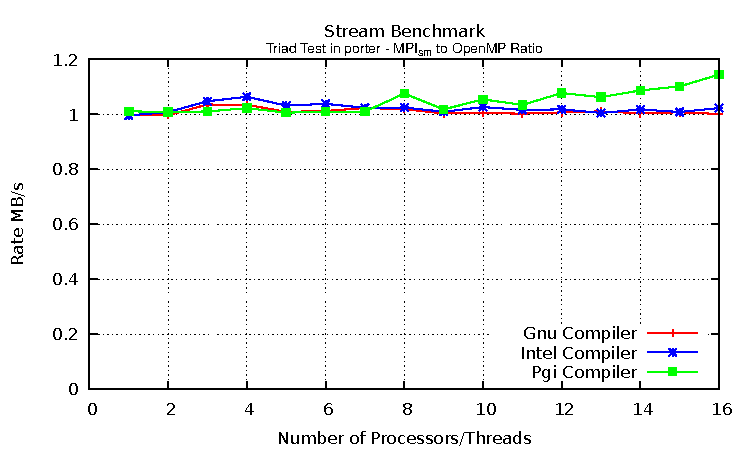
\includegraphics[width=0.95\linewidth]{Plots/streamBenchmark/porter-TriadRatio.pdf}
      \caption{Ratio MPI$_{sm}$ to OpenMP.}
      \label{fig:TriadRatio}
    \end{subfigure}
\caption{Triad test.}
\label{fig:TriadTest}
\end{figure}

\newpage

\subsection*{Barriers}
%causes a central processing unit (CPU) or compiler to enforce 

A memory barrier is a type of instruction that requires an ordering constraint on memory operations issued before and after it. They are necessary because most modern CPUs employ performance optimizations that can result in out-of-order execution. This reordering of memory operations (loads and stores) can produce incorrect results in parallel programs unless carefully controlled.

\medskip


The efficiency of the barrier implementation could potentially affect the overall performance of parallel programs, including those conforming to the shared memory programming model. Therefore, an effort was made to estimate, as accurate as possible, the time delay produced by the barrier itself. A large difference in the barrier delay between MPI$_{sm}$ and OpenMP could result determinant in choosing one or the other.

\medskip

Notice that what is being measured is not the time a particular thread/process takes between entering and exiting
the barrier because that time includes the time spent in the barrier waiting for its partners to arrive. Instead, the parameter being measured correspond to the time elapsed between the last thread/process entering the barrier to the moment in which all of them exit the barrier\cite{Schmidt_2012}. Therefore, this parameter can be approximated by the minimum time taken by all the thread/process between entering and exiting the barrier. Notice also that the parameter being measured is rather small and, therefore, its value is better represented by an average taken over a relatively large amount of measurements.


\medskip

Figure \ref{fig:PseudoCode3} presents a pseudo code of the algorithm used to determine the cost of the barrier in the MPI$_{sm}$ case; the algorithm for OpenMP case is essentially the same and, therefore, is not presented here. In lines 1-2 some variables are declared and initialized. Lines 3-13 consist of a \textbf{\texttt{for}} loop used to generate a sufficiently large amount of measurements required by an accurate result. Line 4 contains a barrier used to synchronize all the processes before performing the actual measurement. In lines 6 and 8 start and stop the clock, while line 7 contains the barrier being timed. In line 10, each process gets the time it spends in the barrier which, in general, includes a delay due to waiting for partners to arrive. In lines 11-12, the smallest time among all the processes is obtained and accumulated in the \textbf{\texttt{barrier\_time}} variable. Finally, in line 14 an average for the barrier time is obtained.


\begin{figure} [t!]
\centering
\captionsetup{justification=centering, singlelinecheck=false}
\begin{lstlisting}[style=CStyle]
uint64_t max_iterations = 1000000L;
uint64_t time, barrier_time=0;
for (uint64_t n=0 ; n<max_iterations; ++n) {
    MPI_Barrier(sm_comm);
        
    clock_gettime(CLOCK_MONOTONIC, &start);
    MPI_Barrier(sm_comm);    
    clock_gettime(CLOCK_MONOTONIC, &end);
    
    time = 1000000000L * (end.tv_sec - start.tv_sec) + end.tv_nsec - start.tv_nsec;
    MPI_Allreduce( MPI_IN_PLACE, &time, 1, MPI_UNSIGNED_LONG, MPI_MIN,sm_comm);
    barrier_time+=time;
}	// end for //
barrier_time/=(max_iterations);
\end{lstlisting}    
\caption{Pseudo used to estimate MPI$_{sm}$ barrier time.}
\label{fig:PseudoCode3}
\end{figure}


\medskip

Figure \ref{fig:BarrierAndErrorBarsForStout} shows result obtained on one system (stout). The left plot (\ref{fig:BarrierStout}) presents average barrier time, in nanoseconds, as a function of the number of threads/processes. The right plot (\ref{fig:BarrierErrorBarsStout}) shows that the variability of those measurements is relatively small.

\medskip

Figure \ref{fig:BarrierStout} expose some contradictory results. While for the Gnu compiler the barrier time taken by OpenMP is larger than its corresponding MPI$_{sm}$ counterpart for any number of processes/threads, for the other two compilers (Intel and PGI) the opposite is true. 




%The results shown here for the stout system are similar to results obtained in the other systems used in this study.


\begin{figure} [h!]
    \centering
    \captionsetup{justification=centering, singlelinecheck=false}
    \begin{subfigure}{.6\textwidth}
      \centering
      \hspace*{-1.5cm} 
      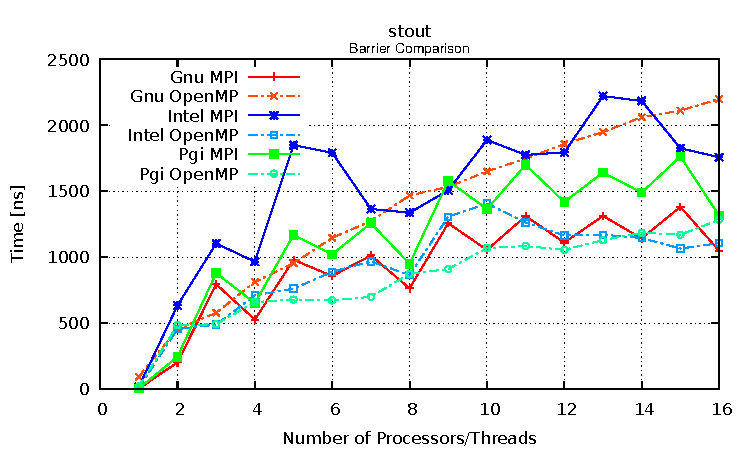
\includegraphics[width=0.95\linewidth]{Plots/barrier/stout.pdf}
      \caption[]{Estimated time.}
      \label{fig:BarrierStout}
    \end{subfigure}%
    \begin{subfigure}{.6\textwidth}
      \centering
      \hspace*{-1.5cm} 
      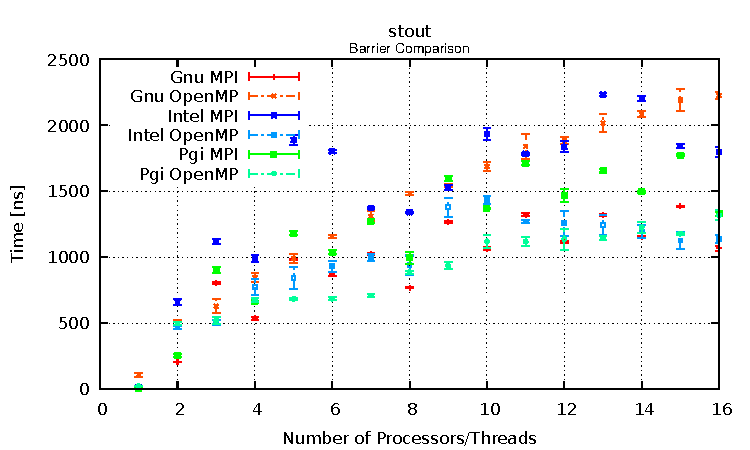
\includegraphics[width=0.95\linewidth]{Plots/barrier/stoutError.pdf}
      \caption{Errorbars to show variability of results.}
      \label{fig:BarrierErrorBarsStout}
    \end{subfigure}
\caption{Barrier Results.}
\label{fig:BarrierAndErrorBarsForStout}
\end{figure}

\medskip

Figure \ref{fig:BarrierAndErrorBarsForKoelsch} presents results obtained in another system (koelsch). In this system, the OpenMP barrier time is always smaller than its MPI$_{sm}$ counterpart.

\medskip



\subsection*{Summary}

In this section two technical aspects that can potentially affect the overall performance of parallel applications conforming to the shared memory programming model (OpenMP and MPI$_{sm}$) were evaluated.

\medskip

Results show that: 

\begin{itemize} 

    \item the sustainable memory bandwidth obtained using MPI$_{sm}$ is as high as that obtained using OpenMP.

    \item The time taken by the OpenMP barrier is, in general, smaller that its MPI$_{sm}$ counterpart. However, we notice that there could be some variability from system to system. Perhaps it is more important to notice that the time taken by these barriers are \textbf{not} orders of magnitude apart.

\end{itemize}


\medskip


\begin{figure} [t!]
    \centering
    \captionsetup{justification=centering, singlelinecheck=false}
    \begin{subfigure}{.6\textwidth}
      \centering
      \hspace*{-1.5cm} 
      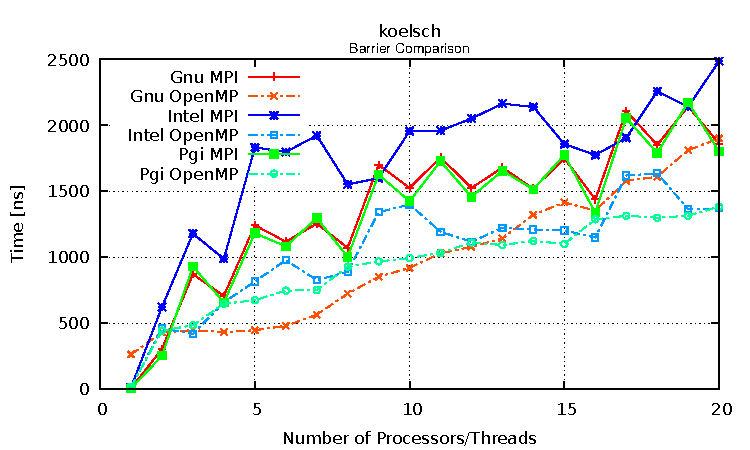
\includegraphics[width=0.95\linewidth]{Plots/barrier/koelsch.pdf}
      \caption[]{Estimated time.}
      \label{fig:BarrierKoelsch}
    \end{subfigure}%
    \begin{subfigure}{.6\textwidth}
      \centering
      \hspace*{-1.5cm} 
      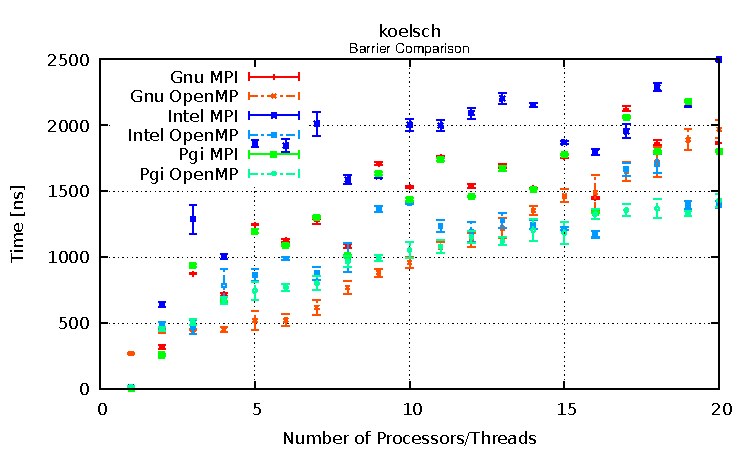
\includegraphics[width=0.95\linewidth]{Plots/barrier/koelschError.pdf}
      \caption{Errorbars to show variability of results.}
      \label{fig:BarrierErrorBarsKoelsch}
    \end{subfigure}
\caption{Barrier Results.}
\label{fig:BarrierAndErrorBarsForKoelsch}
\end{figure}


